\section{Experiments}
\label{sec:experiment}
\subsection{Datasets}
We evaluate our system on several datasets. These datasets offer a wide range of inductive reasoning tasks such as 1D grid manipulation, list operations, causal induction abilities, and sequence-to-sequence operations. We randomly select 10\% of the tasks from each dataset for testing and use the rest for constructing an augmented dataset for model tuning. The data augmentation is performed with GPT-4o as the teacher model, using a hypothesis search size of 50. The statistics of the training data are shown in Table~\ref{tab:dataset_summary}. Details regarding the hypothesis quality within the dataset is shown in Figure~\ref{fig:data_quality} in Appendix~\ref{app:data_quality}.

\begin{table}
\small
\centering
\begin{tabular}{@{}lrrrr@{}}
\toprule
\textbf{} & \textbf{Preference Data} & \textbf{SFT Data} & \textbf{SFT Data} & \textbf{SFT Data} \\ \midrule
\textbf{Tasks} & \textbf{Rule Generation} & \textbf{Rule Generation} & \textbf{Rule Following} & \textbf{Direct Few-shot} \\ \midrule
List Function & 31,186 & 10,514 & 22,568 & 1,800 \\
1D ARC & 38,717 & 20,250 & 17,661 & 810 \\
ACRE & 19,461 & 4,472 & 17,760 & 360 \\ 
SCAN & 19,404 & 4,500 & 30,380 & 900 \\ \midrule
Total & 108,768 & 39,736 & 88,369 & 3,870 \\ \bottomrule
\end{tabular}
\caption{Training Data Statistics}
\label{tab:dataset_summary}
\vspace{-1em}
\end{table}

\paragraph{List Function} \citet{rule2020child} proposed the List Function dataset to provide insight into children's learning abilities from a computer programming perspective. The dataset contains 250 tasks, with both input and output examples provided. Each task comprises eight training and eight test examples, making them suitable for few-shot prompting scenarios. The list operations that map inputs to outputs include operations such as selection, duplication, sorting, and more.

\paragraph{1D ARC} The Abstraction and Reasoning Corpus (ARC)~\citep{chollet2019measureintelligence} is a dataset designed to evaluate machine learning models on complex reasoning and generalization tasks. Each problem in ARC consists of a set of input-output grid-based examples ($30\times30$) and a test input grid. The goal is to infer the transformation pattern and apply it to the test input in order to generate the correct output. The 1D ARC dataset~\citep{xu2024llmsabstractionreasoningcorpus} is a simplified variant of ARC where problems are structured in a one-dimensional format instead of a 2D grid. It retains the core principles of ARC but restricts the input and output examples to linear sequences ($1\times30$) rather than spatial grids.

\paragraph{ACRE} The Abstract Causal REasoning (ACRE)~\citep{zhang2021acreabstractcausalreasoning} dataset is a benchmark designed to evaluate and enhance the causal induction capabilities of visual reasoning systems. Inspired by the ``Blicket'' experiments from developmental psychology, ACRE assesses how well AI models can infer causal relationships beyond mere statistical associations.

\paragraph{MiniSCAN} MiniSCAN~\citep{lake2019humanfewshotlearningcompositional} is a sequence-to-sequence task where an input sequence corresponding to the instruction is transformed into an output action sequence. The instruction is composed of primitive pseudo-words, and the output action sequence consists of colored circles.

\subsection{Baselines \& Metrics}

\paragraph{Baseline Input-to-Output (IO)} This baseline involves a simple few-shot prompting approach without any intermediate reasoning steps. Prompting is performed on frozen language models. Decoding is performed with a temperature of $0.7$ and a top-p of $1.0$. The prompts associated with direct few-shot prompting are shown in Table~\ref{tab:prompts} in Appendix~\ref{app:prompts}. 

\paragraph{Baseline Hypothesis Search (HS)} Following \citet{wang2023hypothesis}, we use the hypothesis search on frozen language models as a baseline. The first step is to generate multiple hypotheses for inductive reasoning that may explain the demonstrated ICL examples. The hypothesis that best fits the examples is chosen. The second step involves applying the hypothesis to a novel input to produce the output. The decoding temperature for rule generation and rule following is $0.9$ and $0.7$, respectively, with top-p set to $1.0$. The prompts associated with hypothesis search are shown in Table~\ref{tab:prompts} in Appendix~\ref{app:prompts}. 

\paragraph{Baseline Input-to-Output with SFT} This baseline involves simple few-shot prompting using models that have been fine-tuned in a multi-task setting. We fine-tune the base models using the data presented in the last column of Table~\ref{tab:dataset_summary}. Training is performed using LoRA (rank $8$, scaling factor $16$). We tune the models for 3 epochs with a learning rate of $10^{-4}$ using the Adam optimizer. The decoding temperature during inference is $0.7$ with a top-p of $1.0$. 

\paragraph{Metrics} 
Raw accuracy is used as the evaluation metric for performance. It is defined as the fraction of correctly predicted ICL outputs with respect to the total number of outputs in the test set. We use the cost-to-performance ratio (CP) as a metric to measure efficiency. CP is defined as the ratio of average token consumption per output to accuracy.


\subsection{Training Details}
We use three language models for our experiments: Llama-3-8B-Instruct~\citep{grattafiori2024llama3herdmodels}, Mistral-7B-Instruct-v0.3~\citep{jiang2023mistral7b}, and Qwen2.5-7B-Instruct~\citep{bai2023qwentechnicalreport}. We perform supervised fine-tuning on both rule generation and rule following, and then perform alignment on preferred rule generation. Supervised fine-tuning is performed using LoRA adaptation with a rank of $8$ and a scaling factor of $16$. The models are fine-tuned for 4 epochs with a learning rate of $10^{-4}$. Alignment is also performed using LoRA adaptation with a rank of $8$ and a scaling factor of $16$. During alignment, we fine-tune the models for 5 epochs with a learning rate of $5\times 10^{-6}$. Training is performed using $2\times 48$~GB Nvidia RTX A6000 GPUs with a per-device batch size of $1$ and gradient accumulation steps of $8$. The durations of SFT and alignment are 48 and 72 hours, respectively. As shown in Table~\ref{tab:main_result}a, we experiment with different combinations of SFT and alignment for Llama-3-8B-Instruct. We then apply the best-performing combination to the two remaining models.

During inference with \proposed, we set a decoding temperature of $0.9$ for rule generation and $0.7$ for rule following, with a top-p set to $1.0$. The best decoding temperatures are estimated with a grid search, as shown shown in Figure~\ref{fig:temperature_search} in Appendix~\ref{app:temperature}. Unless otherwise specified, we use the same model checkpoint for rule generation and rule following during inference.

\begin{table}
\resizebox{\textwidth}{!}{
\begin{tabular}{lllrrrrr}
\toprule
& \textbf{Method} & \textbf{Tuning} & \textbf{List Func} & \textbf{1D ARC} & \textbf{ACRE} & \textbf{MiniSCAN} \\ \midrule
\multirow{5}{*}{a)} & Baseline IO & N/A & $0.43\pm0.01$ & $0.07\pm 0.01$ & $0.53\pm 0.01$ & $0.10\pm 0.01$ \\
& Baseline IO & SFT (Few-shot) &  $0.47\pm 0.01$ &  $0.40\pm 0.01$ &  $0.70\pm 0.01$ &  $0.25\pm 0.01$ \\
& Baseline HS & N/A &  $0.36\pm 0.01$ &  $0.04\pm 0.01$ &  $0.08\pm 0.01$ &  $0.00\pm 0.00$ \\
& \multirow{5}{*}{\proposed-Llama} & SFT (RG+RF)\footnotemark[1] &  $0.43\pm 0.00$ &  $\underline{0.47}\pm 0.00$ &  $0.65\pm 0.00$ &  $0.21\pm 0.00$ \\
&  & SFT (RG+RF) + DPO (RG) &  $\textbf{0.49}\pm 0.01$ &  $\underline{0.51}\pm 0.01$ &  $\underline{\textbf{0.73}}\pm 0.01$ &  $\underline{0.42}\pm 0.01$ \\
& & SFT (RG+RF) + ORPO (RG)\footnotemark[1] & $\textbf{0.49}\pm 0.01$ & $\underline{\textbf{0.53}}\pm 0.01$ & $\underline{\textbf{0.73}}\pm 0.01$ & $\underline{\textbf{0.45}}\pm 0.01$ \\
&  & SFT (RG+RF)+ KTO (RG) &  $0.48\pm 0.01$ &  $\underline{0.51}\pm 0.01$ &  $0.72\pm 0.01$ &  $\underline{0.38}\pm 0.01$ \\
& & SFT (RF) + ORPO (RG) &  $0.41\pm 0.01$ &  $0.43\pm 0.01$ &  $0.59\pm 0.01$ &  $0.21\pm 0.01$ \\ \midrule 
\multirow{5}{*}{b)} & Baseline IO & N/A & $0.43\pm0.00$ & $0.16\pm 0.01$ & $0.70\pm 0.00$ & $0.04\pm 0.00$ \\
& Baseline IO & SFT (Few-shot) &  $0.44\pm 0.00$ &  $0.17\pm 0.00$ &  $0.73\pm 0.00$ &  $0.25\pm 0.00$ \\
& Baseline HS & N/A & $0.33\pm 0.01$ &  $0.01\pm 0.01$ &  $0.00\pm 0.00$ &  $0.02\pm 0.01$ \\
&\multirow{2}{*}{\proposed-Qwen} & SFT (RG+RF)\footnotemark[1] &  $0.45\pm 0.00$ &  $\underline{0.45}\pm 0.00$ &  $0.68\pm 0.00$ &  $0.19\pm 0.00$ \\
& & SFT (RG+RF) + ORPO (RG)\footnotemark[1] & $\textbf{0.54}\pm 0.01$ & $\underline{\textbf{0.48}}\pm 0.01$ & $\underline{\textbf{0.80}}\pm 0.01$ & $\underline{\textbf{0.43}}\pm 0.01$ \\ \midrule
\multirow{5}{*}{c)} & Baseline IO & N/A & $0.41\pm0.00$ & $0.09\pm 0.01$ & $0.52\pm 0.00$ & $0.08\pm 0.00$ \\
& Baseline IO & SFT (Few-shot) &  $0.42\pm 0.00$ &  $0.27\pm 0.00$ &  $0.75\pm 0.00$ &  $0.22\pm 0.00$ \\
& Baseline HS & N/A &  $0.25\pm 0.01$ &  $0.02\pm 0.01$ &  $0.05\pm 0.01$ &  $0.00\pm 0.00$ \\
&\multirow{2}{*}{\proposed-Mistral} & SFT (RG+RF)\footnotemark[1] &  $0.41\pm 0.00$ &  $0.40\pm 0.00$ &  $0.70\pm 0.00$ &  $0.10\pm 0.00$ \\
& & SFT (RG+RF) + ORPO (RG)\footnotemark[1] & $\textbf{0.45}\pm 0.01$ & $\underline{\textbf{0.53}}\pm 0.01$ & $\underline{\textbf{0.78}}\pm 0.01$ & $\underline{\textbf{0.35}}\pm 0.01$ \\ \midrule
\multicolumn{2}{c}{gpt-3.5-turbo\footnotemark[2] IO} & N/A &  $0.49\pm 0.01$ &  $0.14\pm 0.01$ &  $0.00\pm 0.00$ &  $0.01\pm 0.01$ \\
\multicolumn{2}{c}{gpt-3.5-turbo\footnotemark[2] HS} & N/A &  $0.50\pm 0.01$ &  $0.08\pm 0.01$ &  $0.00\pm 0.00$ &  $0.01\pm 0.01$ \\ \midrule
\multicolumn{2}{c}{deepseek v3 IO} & N/A &  $0.68\pm 0.01$ &  $0.67\pm 0.01$ &  $0.72\pm 0.00$ &  $0.26\pm 0.01$ \\ 
\multicolumn{2}{c}{deepseek v3 HS} & N/A &  $0.61\pm 0.01$ &  $0.40\pm 0.01$ &  $0.00\pm 0.00$ &  $0.04\pm 0.01$ \\ \midrule
\multicolumn{2}{c}{gpt-4o IO} & N/A &  $0.61\pm 0.01$ &  $0.44\pm 0.01$ &  $0.77\pm 0.01$ &  $0.27\pm 0.01$ \\ 
\multicolumn{2}{c}{gpt-4o HS} & N/A &  $0.69\pm 0.01$ &  $0.43\pm 0.01$ &  $0.71\pm 0.01$ &  $0.27\pm 0.01$ \\ \bottomrule
\end{tabular}
}
\caption{Performance of \proposed is evaluated using the following models: (a) Llama-3-8B-Instruct, (b) Qwen2.5-7B-Instruct, and (c) Mistral-7B-Instruct. IO refers to direct input-to-output few-shot prompting, and HS refers to the hypothesis search method. Both the hypothesis search baselines and \proposed use a hypothesis size of 10. RG and RF refer to rule generation and rule following, respectively. Underlined results indicate cases where a variant of \proposed outperforms GPT-4o with hypothesis search.
}
\label{tab:main_result}
\end{table}

\footnotetext[1]{We will refer to the SFT (RG+RF) + ORPO (RG) variant of \proposed model simply as \proposed and SFT (RG+RF) variant of \proposed model as SFT.}
\footnotetext[2]{gpt-3.5-turbo-1106}

\subsection{Results}
\paragraph{Comparison with baselines} Table~\ref{tab:main_result} shows the performance of \proposed compared to three baselines, across several open-weight models. \proposed outperforms the three baselines for each base model. In particular, \proposed performs better than the strongest few-shot prompting baseline, which has been fine-tuned for the few-shot ICL setting on the same tasks. For example, \proposed-Qwen achieves 23\%, 182\%, 9\%, and 72\% relative improvement over Baseline IO-SFT on List Function, 1D ARC, ACRE, and MiniSCAN, respectively. This demonstrates that reasoning distillation, which teaches the student model the underlying rules, is more effective than direct input-output ICL distillation, as the latter may not generalize well to novel inputs.

\paragraph{Comparison with the teacher} The \proposed model outperforms the teacher model, GPT-4o, on three out of four tasks across all three base models. For example, \proposed-Llama achieves relative improvements of 23.2\%, 2.8\%, and 66.6\% over GPT-4o for 1D ARC, ACRE, and MiniSCAN, respectively, when both models use a hypothesis search size of 10. This improvement can be attributed to the difference in hypothesis size during data augmentation and inference, as well as the impact of data filtering, SFT, and alignment. We performed data augmentation with a hypothesis size of 50. During data filtering, some low-quality rules in the candidate space are filtered out. Thus, the SFT stage helps the student model generate higher-quality rules compared to the teacher within an equivalent candidate set. The alignment stage further ensures that the best candidates are among the top candidates generated by the distilled model. Consequently, the distilled model with a smaller hypothesis search space can mimic the performance of the teacher model with a larger hypothesis search space.

\paragraph{Impact of SFT and Alignment Combinations} For \proposed-Llama, we first perform SFT on rule generation and rule-following. We then apply three preference alignment strategies to the fine-tuned model individually: DPO, ORPO, and KTO. We find that ORPO achieves the best performance, outperforming DPO on 1D ARC and MiniSCAN by two and three percentage points, respectively. While the SFT loss during initial fine-tuning jointly optimizes both rule generation and rule-following, the SFT loss within ORPO exclusively optimizes rule generation. Therefore, we hypothesize that the SFT loss component in ORPO contributes to the additional improvement. Since \citet{hong2024orpomonolithicpreferenceoptimization} originally proposed ORPO to circumvent the need for a separate SFT stage, we experiment with a variant in which SFT is performed on rule-following only. ORPO is then applied to rule generation (the last row of Table~\ref{tab:main_result}a). We find that this variant underperforms even compared to the SFT-only version. This indicates that if the discrepancy between the rule quality generated by the teacher and the base student model is too large, ORPO alone cannot eliminate the need for fine-tuning on rule generation.

\begin{figure}
\centering
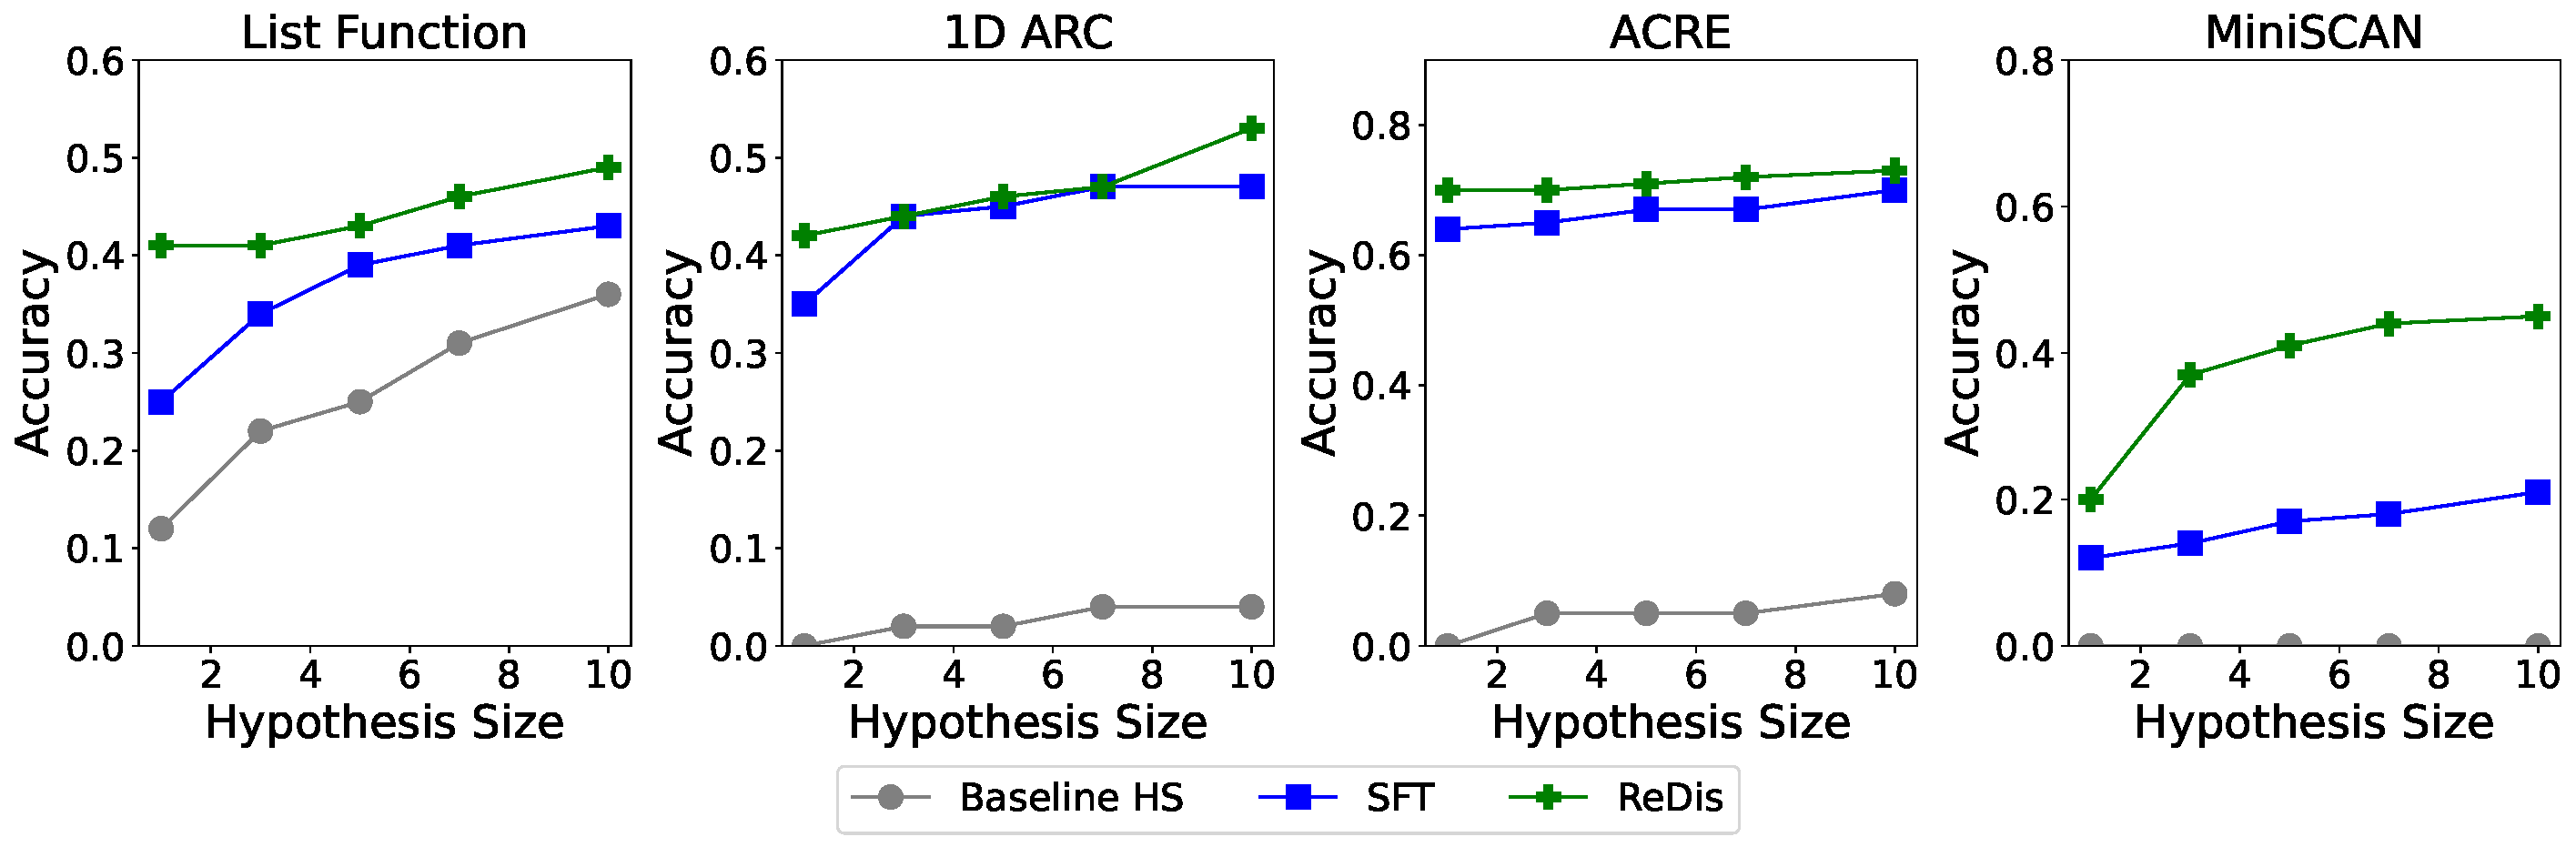
\includegraphics[width=\textwidth]{Figures/accuracy_hypo.pdf}
\caption{The impact of hypothesis size on performance improvement of \proposed-Llama. The results are shown for hypothesis size of $1, 3, 5, 7,$ and $10$.}
\label{fig:accuracy_hypo}
\end{figure}

\paragraph{Impact of Hypothesis Size} Figure~\ref{fig:accuracy_hypo} shows the impact of hypothesis size on \proposed-Llama performance. We find that the aligned model performs better than the base model and the SFT-only variant across all hypothesis sizes. The performance gap is more prominent for a very small candidate set, as demonstrated in the case of List Function and 1D ARC tasks for the hypothesis size of one. This indicates that preference alignment can help the student model generate better rules at the top of the candidate list.

\begin{table}
\small
\centering
\begin{tabular}{lrrrrrrrrr}
\toprule
Models & $m$ & \multicolumn{2}{c}{List Func} & \multicolumn{2}{c}{1D ARC} & \multicolumn{2}{c}{ACRE} & \multicolumn{2}{c}{MiniSCAN} \\ \midrule
&  & Acc\textuparrow & CP\textdownarrow & Acc\textuparrow & CP\textdownarrow & Acc\textuparrow & CP\textdownarrow & Acc\textuparrow & CP\textdownarrow \\
 \midrule
Baseline & 10 & 0.36 & 72 & 0.04 & 73050 & 0.08 & 8287 & 0.00 & -- \\
gpt-3.5-turbo &10 & 0.50 & 469 & 0.08 & 19321 & 0.00 & -- & 0.01 & 27200 \\
gpt-4o &10 & 0.69 & 646 & 0.43 & 8317 & 0.71 & 235 & 0.27 & 4925 \\
deepseek v3 &10 & 0.61 & 1013 & 0.40 & 13272 & 0.00 & -- & 0.04 & 55525 \\
SFT &10 & 0.43 & 625 & 0.47 & 7493 & 0.65 & 210 & 0.21 & 2704 \\
\proposed &10 & 0.49 & \underline{644} & 0.53 & \underline{6611} & 0.73 & 338 & 0.45 & \underline{1095} \\ 
\proposed &5 & 0.43 & \underline{\textbf{393}} & 0.46 & \underline{\textbf{3869}} & 0.71 & \underline{\textbf{176}} & 0.41 & \underline{\textbf{631}} \\ 
\bottomrule
\end{tabular}
\caption{Cost to performance (CP) ratio of \proposed-Llama is compared with the base, fine-tuned, and proprietary models. All models use hypothesis search and $m$ denotes the size of the search space. \proposed variants that outperform GPT-4o is underlined.}
\label{tab:token_consumption}
\end{table}

\paragraph{Inference-time optimization} One significant advantage of the proposed reasoning distillation is the inference-time optimizations it can provide over the teacher model. Table~\ref{tab:token_consumption} shows the cost-to-performance ratio for each test set. \proposed-Llama with top-5 hypotheses achieves 87\%, 53\%, and 25\% relative improvements in cost-to-performance ratio compared to the teacher model for MiniSCAN, 1D ARC, and ACRE, respectively.

\paragraph{Impact of hypothesis length} Interestingly, we find that the \proposed model trained only with SFT sometimes becomes more token-efficient than the teacher model, even when the hypothesis size is the same. For example, the SFT-only variant is 10\% more token-efficient than GPT-4o on the 1D ARC task (shown in Table~\ref{tab:token_consumption}). To investigate this observation, we calculate the Pearson correlation coefficient between hypothesis length and quality. The task- and dataset-specific correlation coefficients are reported in Table~\ref{tab:hypo_len}. We find that longer hypotheses tend to have lower quality scores for the List Function and 1D ARC tasks. It is possible that language models may struggle to follow overly long or complex rules. Therefore, longer hypotheses are automatically removed from the SFT dataset during fitness estimation, and the fine-tuned model prefers shorter hypotheses that are easier to follow.

\begin{table}
\small
\centering
\begin{tabular}{lrrrrr}
\toprule
Attribute & All & List Func & 1D ARC & ACRE & MiniSCAN \\ \midrule
Pearson correlation coefficient & -0.20 & -0.31 & -0.25 & 0.17 & 0.04 \\
Share of SFT Data & 1.00 & 0.26 & 0.51 & 0.11 & 0.12 \\ \bottomrule
\end{tabular}
\caption{Pearson correlation coefficients between hypothesis quality and hypothesis length are shown for all SFT data and task-specific SFT data. We find that longer hypotheses may be associated with lower overall quality in most cases.}
\label{tab:hypo_len}
\end{table}

\begin{table}
\resizebox{\textwidth}{!}{
\begin{tabular}{llcccc}
\toprule
RG Model & RF Model & List Func & 1D ARC & ACRE & MiniSCAN \\ \midrule
SFT (RG+RF) + ORPO (RG) & SFT (RG+RF) + ORPO (RG) & 0.49 & 0.53 & 0.73 & 0.45 \\
SFT (RG+RF) + ORPO (RG) & Base & 0.43 & 0.12 & 0.08 & 0.01 \\
SFT (RG+RF) + ORPO (RG) & SFT (RG+RF) & 0.49 & 0.54 & 0.73 & 0.46 \\
Base & SFT (RG+RF) + ORPO (RG) & 0.39 & 0.17 & 0.55 & 0.09 \\
SFT (RG+RF) & SFT (RG+RF) + ORPO (RG) & 0.45 & 0.46 & 0.68 & 0.21 \\ \bottomrule
\end{tabular}
}
\caption{Ablation Study for \proposed-Llama, for hypothesis size of $10$.}
\label{tab:ablation}
\end{table}

\paragraph{Ablation Study} During the ablation study, we use separate checkpoints for rule generation and rule following to determine the impact of SFT and alignment on each reasoning step separately, as shown in Table~\ref{tab:ablation}. The first row indicates our default setup, where the same model is used for both reasoning steps. The most significant performance drop occurs when rule following is performed with a base LLaMA model. For example, we see a 77\% relative drop in accuracy for the 1D ARC task. This indicates that fine-tuning on rule following is critical for optimal performance, as this allows the system to evaluate and select the best hypothesis during hypothesis search. We also find that performing alignment on rule generation with a low-rank adaptation does not degrade the rule-following ability of the models, as the performance is comparable to the ablation scenario where the SFT-only model is used for rule following. We see a 68\% drop in accuracy when the base model is used for rule generation and a 13\% drop when only alignment is removed for the rule generation model. Therefore, SFT on rule generation is the second most critical factor in \proposed's performance, followed by alignment on rule generation.

